\documentclass[xcolor=dvipsnames,handout]{beamer}

\newcommand\NN{\mathbb{N}}
\newcommand\ZZ{\mathbb{Z}}
\newcommand\QQ{\mathbb{Q}}
\newcommand\RR{\mathbb{R}}
\newcommand\CC{\mathbb{C}}
\newcommand\AF{\mathbb{A}}
\newcommand\PP{\mathbb{P}}
\newcommand\FF{\mathbb{F}}
\newcommand\bb{\mathbb}
\newcommand\dr{\mathrm}
\newcommand\kal{\mathscr}
\newcommand\fk{\mathfrak}
\newcommand\op{\oplus}
\newcommand\ot{\otimes}
\newcommand\ds{\displaystyle}
\newcommand\id{\indent}
\newcommand\nid{\noindent}
\newcommand\seq{\subseteq}
\newcommand\sneq{\subsetneq}
\newcommand\speq{\supseteq}
\newcommand\spneq{\supsetneq}
\newcommand\rar{\rightarrow}
\newcommand\Rar{\Rightarrow}
\newcommand\xrar{\xrightarrow}
\newcommand\lar{\leftarrow}
\newcommand\Lar{\Leftarrow}
\newcommand\xlar{\xleftarrow}
\newcommand\lrar{\leftrightarrow}
\newcommand\Lrar{\Leftrightarrow}
\newcommand\ideal{\trianglelefteq}
\newcommand\such{\text{ s.t. }}
\newcommand\sk{(\textit{Sketch}) }
\newcommand\rhup{\rightharpoonup}
\newcommand\rhdn{\rightharpoondown}
\newcommand\lhup{\leftharpoonup}
\newcommand\lhdn{\leftharpoondown}
\newcommand\incl{\hookrightarrow}
\newcommand\vid{\emptyset}
\newcommand\wt{\widetilde}
\newcommand\wh{\widehat}
\newcommand\ol{\overline}
\newcommand\Lor{\Longrightarrow}
\newcommand\Lol{\Longleftarrow}
\newcommand\Lolr{\Longleftrightarrow}
\newcommand\ld{{}^\ast}
\newcommand\lgr{{}^{\ast-\text{gr}}}
\newcommand\kap{\Bbbk^a[\kal{P}]}
\newcommand\kcp{\Bbbk^c[\kal{P}]}
\newcommand\fc{\mathfrak{c}}
\newcommand\qq{\enquote}
\newcommand\coli{\protect\varinjlim}
\newcommand\li{\protect\varprojlim}
\newcommand\injr{\rightarrowtail}
\newcommand\surjr{\twoheadrightarrow}
\newcommand\injl{\leftarrowtail}
\newcommand\surjl{\twoheadleftarrow}
\newcommand\sqsb{\sqsubseteq}

\usepackage{listings}
\usepackage{color}
\lstdefinestyle{mystyle}{
  backgroundcolor=\color{white},   
  commentstyle=\color{gray},
  keywordstyle=\color{blue},
  numberstyle=\tiny\ttfamily,
  stringstyle=\color{olive},
  basicstyle=\small\ttfamily,
  breakatwhitespace=false,         
  breaklines=true,                 
  captionpos=b,                    
  keepspaces=true,                 
  numbers=left,                    
  numbersep=5pt,                  
  showspaces=false,                
  showstringspaces=false,
  showtabs=false,                  
  tabsize=4
}

\lstset{style=mystyle}
\renewcommand{\lstlistingname}{Codul}
\usepackage{soul}
\newcommand{\code}[1]{\texttt{#1}}
\soulregister{\code}{1}

% font setup
\usepackage{libertine}
\usepackage{libertinust1math}
\renewcommand*\familydefault{\sfdefault}    % Linux Libertine = default sans serif
\usepackage{inconsolata}                    % Inconsolata = monospaced
\usepackage[utf8]{inputenc}
\usepackage[T1]{fontenc}
\usepackage{mathrsfs}

% Graphics and other packages
\usepackage[romanian]{babel}
\usepackage{graphicx}
\addto\captionsromanian{\renewcommand{\figurename}{Ilustrație}}
\usepackage{caption}
\usepackage{subcaption}
\usepackage[style=german]{csquotes}

% Custom macros
\newtheorem{bl}{}
\newcommand{\bloc}[3]{\begin{bl}<#1->{{\large\color{Gray}{\hrulefill}}\\ \color{bleumarin}{\large \emph{#2}}}\\ \vspace*{-2mm}{\color{Gray}{\hrulefill}}\\ #3 \end{bl}} 
\newcommand{\fr}[1]{\frame{#1}}
\newcommand{\ft}[1]{\frametitle{\color{bleumarin}{\hfill #1 \hfill}}}
\newcommand{\lin}[3]{\uncover<#1->{\alert<#1>{#2}}{\vspace*{#3 ex}}}
\newcommand{\ite}[2]{\uncover<#1->{\alert<#1>{\item #2}}}
\newcommand{\vs}[1]{\vspace*{#1 ex}}
\definecolor{bleumarin}{RGB}{30,30,150} 
\definecolor{firebrick}{RGB}{178,34,34}

% Theme setup
\useoutertheme{shadow} 
\usetheme{CambridgeUS} 
\usecolortheme[named=bleumarin]{structure} 
\useoutertheme[compress]{smoothbars}

% Theme finetuning
\setbeamertemplate{items}[ball]
\setbeamertemplate{blocks}[rounded][shadow=true]
\setbeamertemplate{navigation symbols}{}
\setbeamertemplate{headline}{}  


%%%%%%%%%%%%%%%%%%%%%%%%%%%%%%%%%%%%%%%%%%%%%%%%%%%%%%%%%%%%%%%%%%%%%% 
% TITLE PAGE
\title[\code{Monocypher} + {FramaC/Eva}]{Verificarea \code{Monocypher} cu \code{FramaC/Eva}}
\author{Adrian Manea}
\institute{SLA, 410}

\date{}

\begin{document}

\maketitle
%%%%%%%%%%%%%%%%%%%%%%%%%%%%%%%%%%%%%%%%%%%%%%%%%%%%%%%%%%%%%%%%%%%%%% 


% SLIDES START HERE
\fr{
  \ft{Uneltele de verificare}

  \lin{1}{\code{FramaC} --- implementat în OCaml, pentru verificarea programelor C.}{0}

  \lin{2}{Oferă o verificare automată sau cu adnotări în ACSL.}{0}

  \lin{3}{Face doar verificări \qq{de bază}. Extins prin plugin-uri:}{0}
  \begin{itemize}
    \ite{4}{\code{WP} = Weakest Precondition calculus;}
    \ite{5}{\code{RTE} = RunTime Evaluation;}
    \ite{6}{\code{Eva} = Evolved Value Analysis;}
    \ite{7}{poate integra demonstratorul \code{Coq}.}
  \end{itemize}

  \lin{8}{Detalii: \cite{acsl}, \cite{framac}, \cite{eva}.}{0}
}



\fr{
  \ft{Exemplu: \code{FramaC} CLI + GUI}
  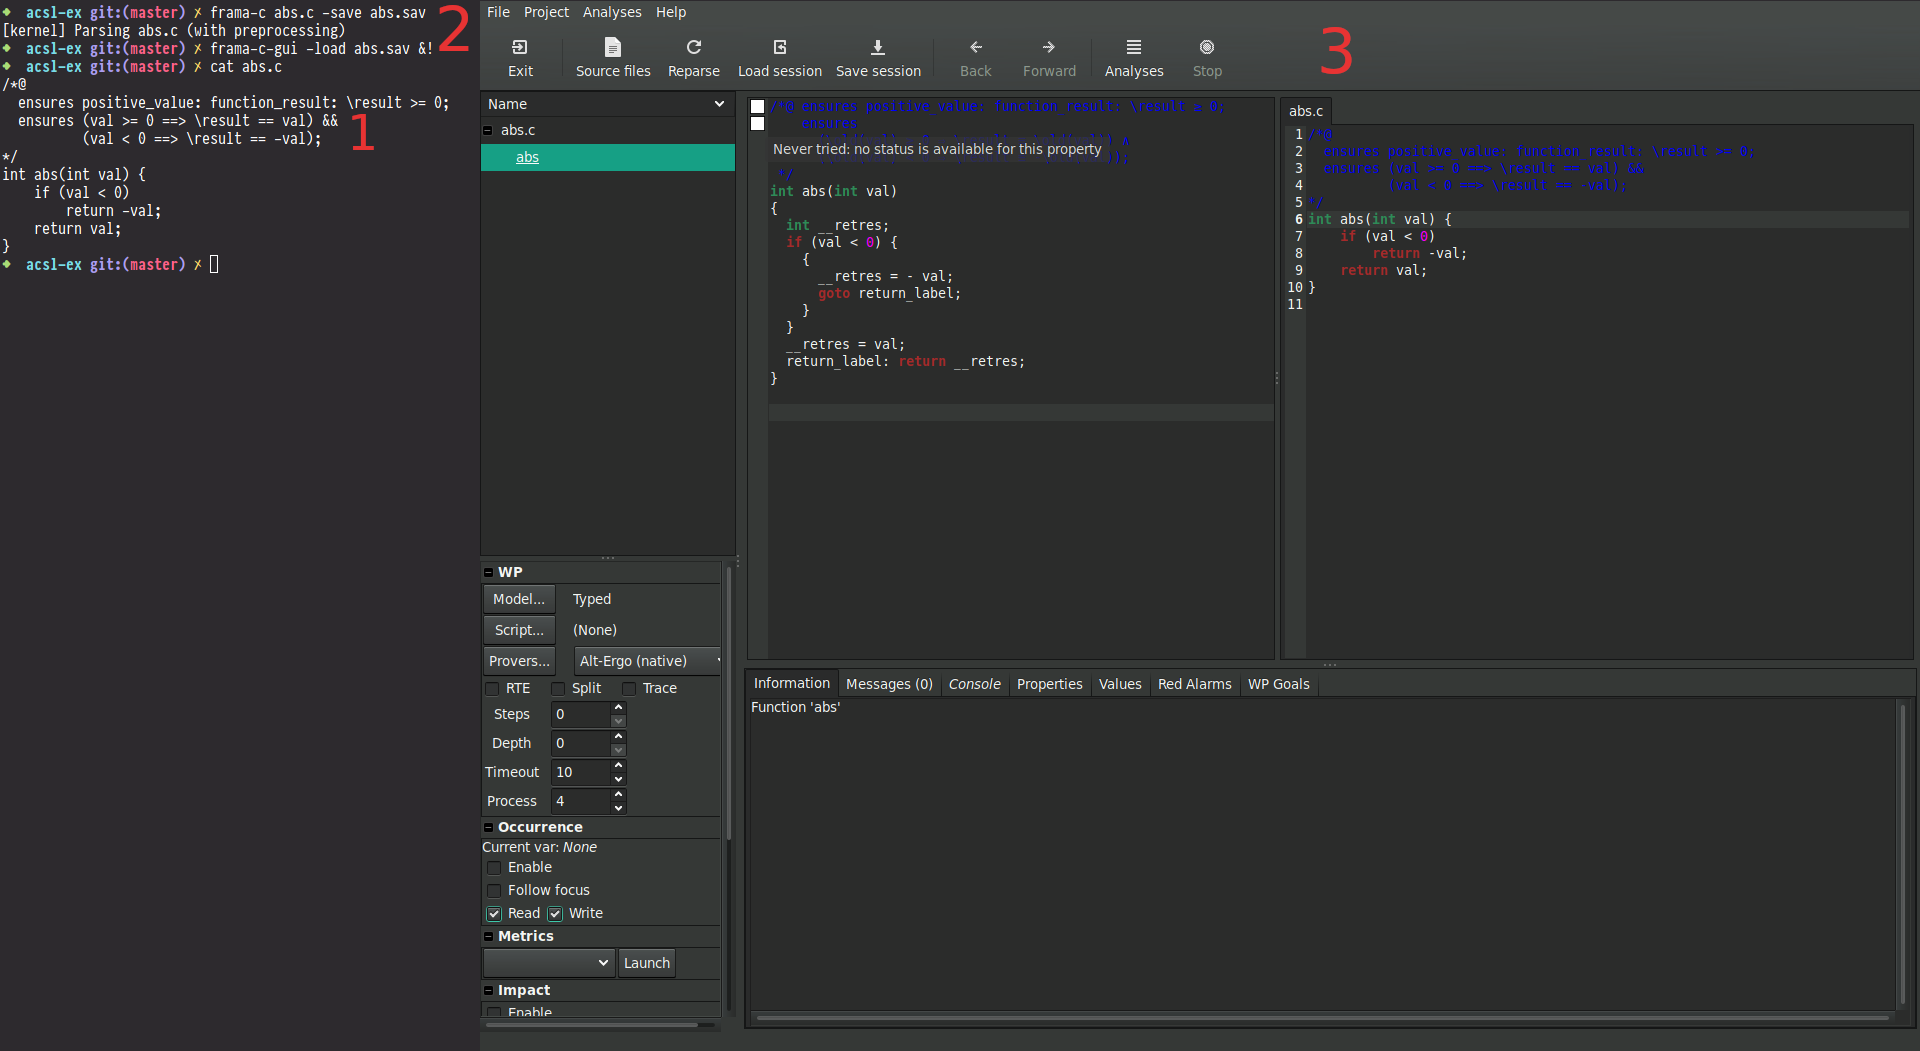
\includegraphics[width=1\textwidth]{../latex/img/exemplu.png}
}

\fr{
  \ft{\code{Eva}}

  \lin{1}{Bazat pe \textbf{interpretarea abstractă} (\cite{abs}).}{2}

  \lin{2}{Ideea: pornind de la \emph{semantica concretă} a unei bucăți de cod,
    se \emph{abstractizează}, pentru ușurarea calculelor.}{2}

  \lin{3}{\code{Eva} calculează valorile și intervalele valorilor unor variabile.}{2}

  \lin{4}{Face sub- sau supra-aproximări, deci produce \emph{alarme}, nu erori.}{2}
}

\fr{
  \ft{\code{Monocypher}}

  \lin{1}{Este o bibliotecă criptografică simplă și rapidă. (\cite{gh1})}{2}

  \lin{2}{Folosește algoritmi criptografici clasici: \code{sha\_512}, \code{ChaCha20} (\cite{monosite},
    \cite{loupcrypto}).}{2}
}

\begin{frame}[fragile]
  \ft{Rularea inițială}

\begin{verbatim}
      # rezultate stdout:
      $ frama-c *.c
      # rezultate log
      $ frama-c *.c > log ; cat log | less
      # rezultate salvate, apoi GUI
      $ frama-c *.c -save firstrun.sav
      $ frama-c-gui -load firstrun.sav
\end{verbatim}

  \lin{2}{Se pot da opțiuni suplimentare de preprocesor și se încarcă în GUI rezultatul, pentru
    a vizualiza mai bine rezultatele.}{2}
\end{frame}

\fr{
  \ft{Rularea inițială în GUI}
  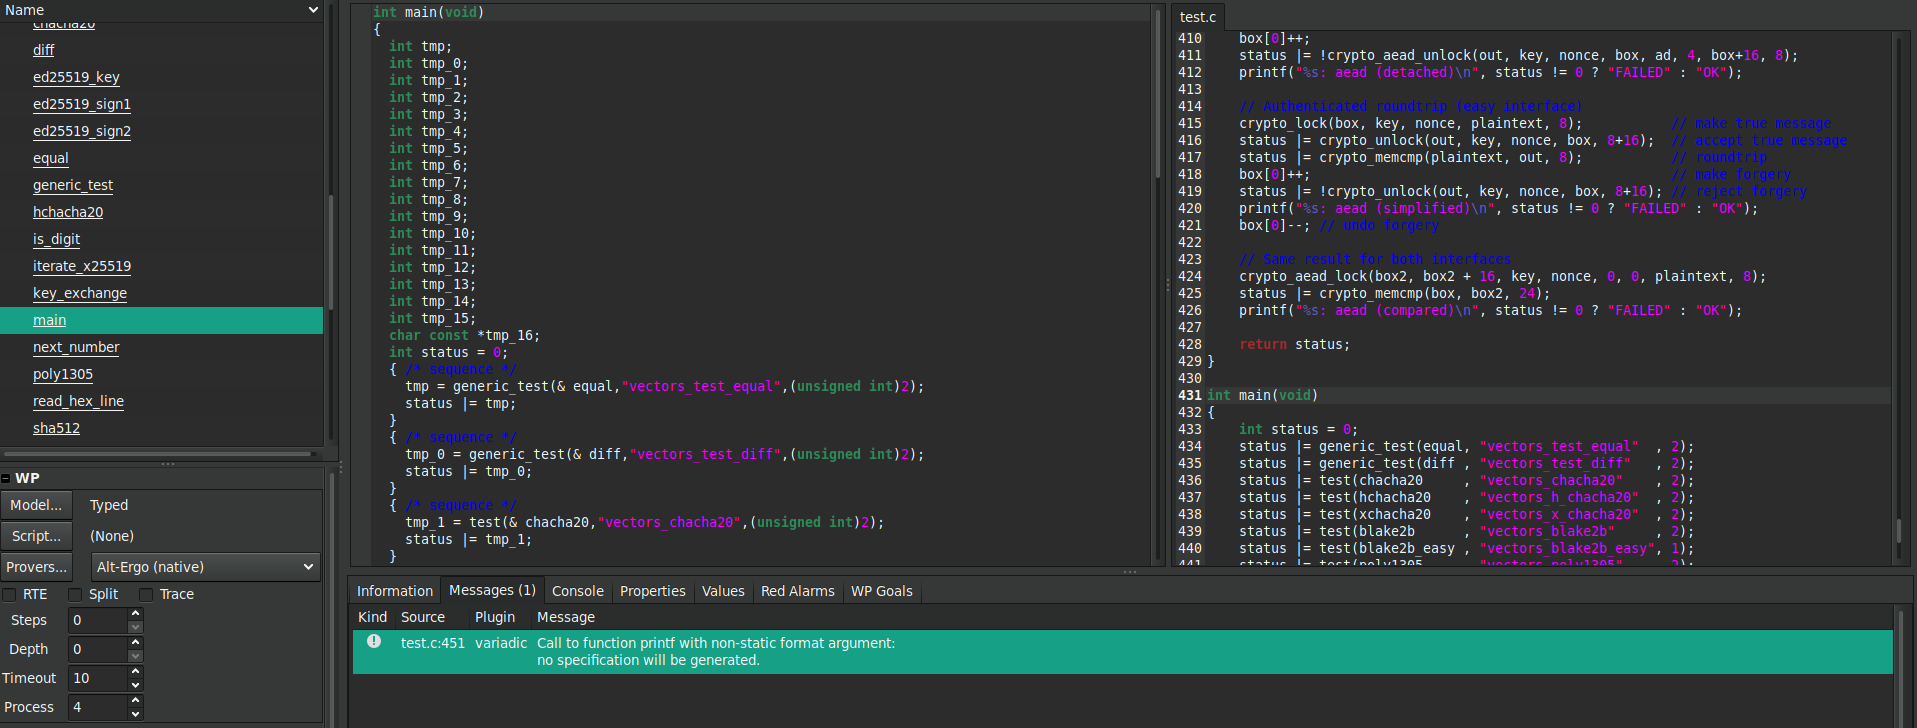
\includegraphics[width=1\textwidth]{../latex/img/framagui1.png}
}

\begin{frame}[fragile]
  \ft{Verificarea cu \code{Eva}}

\begin{verbatim}
$ frama-c -load parsed.sav -val -val-builtins-auto \
          -no-val-show-progress -memexec-all -save value.sav > log
\end{verbatim}

  \begin{itemize}
    \ite{2}{\code{-val} = \code{Eva};}
    \ite{3}{\code{-val-builtins-auto} = verificările standard;}
    \ite{4}{\code{-no-val-show-progress} = nu se afișează mesaje cînd se intră în fiecare funcție;}
    \ite{5}{\code{-memexec-all} = se păstrează în cache valorile calculate, pentru refolosire.}
  \end{itemize}
\end{frame}

\begin{frame}[fragile,allowframebreaks]
  \ft{Cîteva linii din \code{log}}
  \begin{verbatim}
    [value] Analyzing a complete application starting at main
    [value] Computing initial state
    [value] Initial state computed
    [value:initial-state] Values of globals at initialization
    __fc_errno in [--..--]
    __fc_stderr in {{ NULL ; &S___fc_stderr[0] }}
    __fc_strtok_ptr in {0}
    K[0] in {4794697086780616226}
    [1] in {8158064640168781261}
    ...
    blake2b_compress_sigma[0][0] in {0}
    [0][1] in {1}
    ...
    [value:alarm] test.c:126: Warning: 
    out of bounds write. assert \valid(v->buf + v->size);
    [value:alarm] test.c:121: Warning: 
    function memcpy: precondition 'valid_src' got status unknown.
    [value:alarm] monocypher.c:839: Warning: 
    signed overflow. assert g3 * 19 leq 2147483647;
    [kernel] monocypher.c:494: 
    more than 200(253) locations to update in array. Approximating.
\end{verbatim}
\end{frame}

\fr{
  \ft{Rafinarea verificării în GUI}
  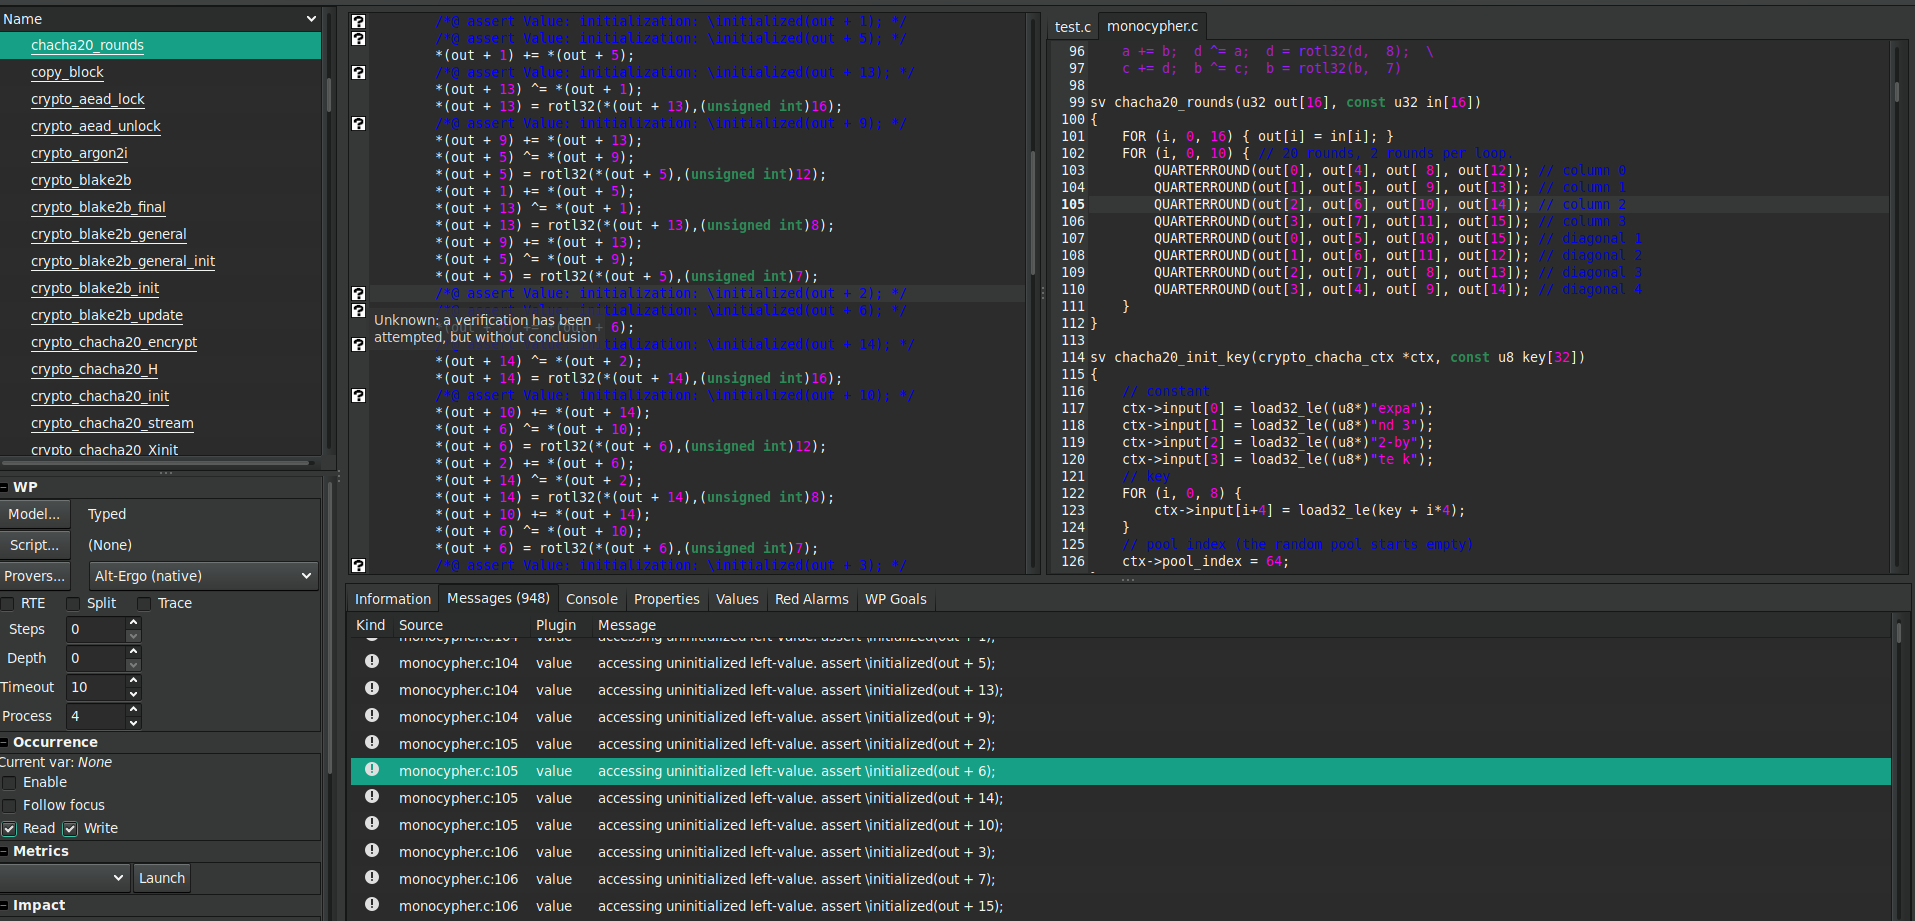
\includegraphics[width=1\textwidth]{../latex/img/framagui2.png}
}

\fr{
  \ft{Rafinarea verificării în GUI}
  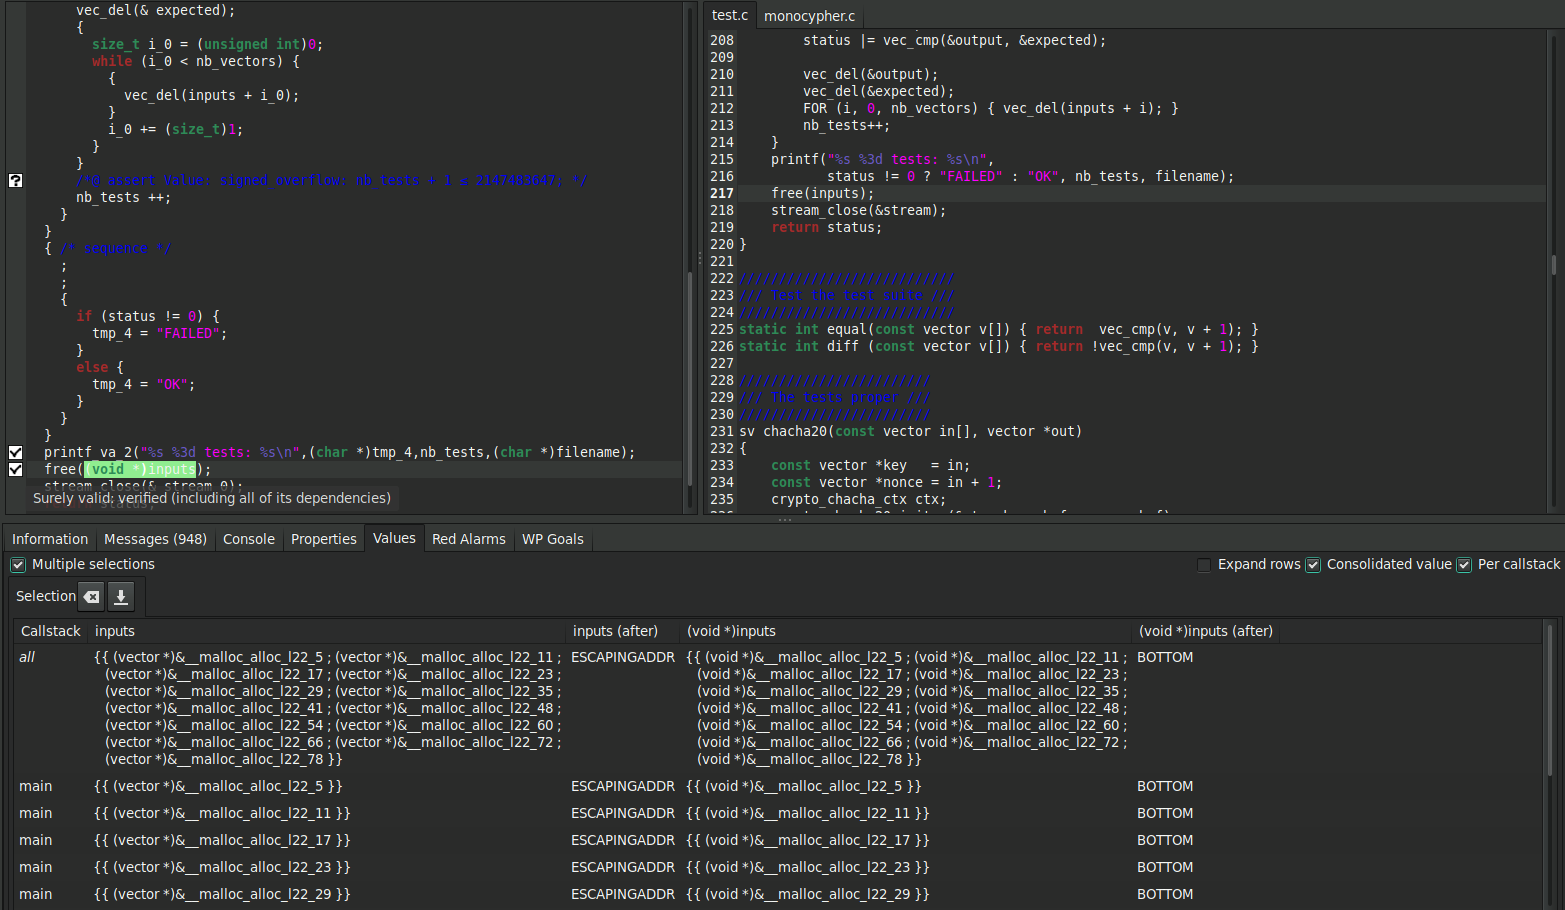
\includegraphics[width=1\textwidth]{../latex/img/framagui3.png}
}

\fr{
  \ft{Concluzii: NO BUGS}
  \lin{1}{Neterminare în versiuni anterioare (\cite{framatut}):}{0}
  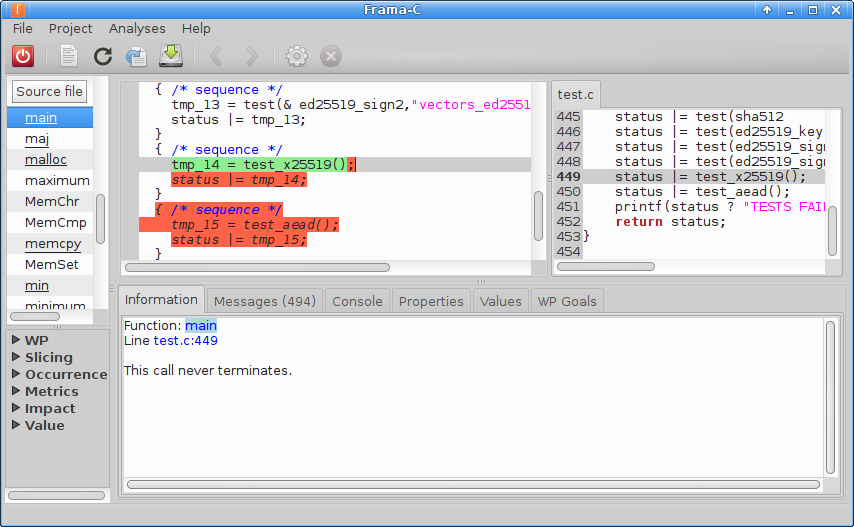
\includegraphics[width=1\textwidth]{../latex/img/nonterm0.png}
}

\fr{
  \ft{Neterminarea în versiuni anterioare}
  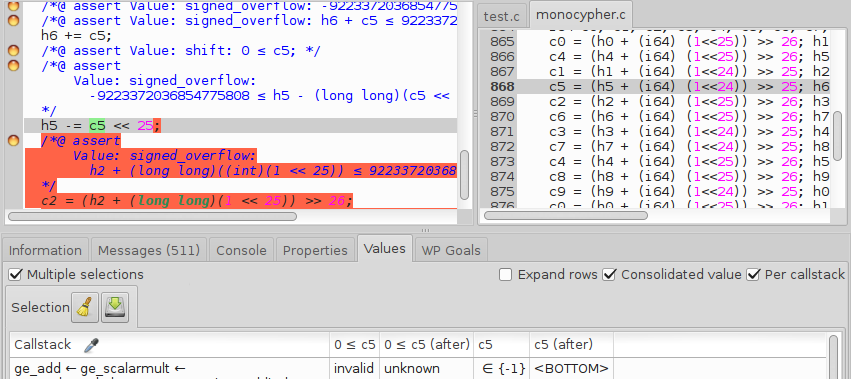
\includegraphics[width=1\textwidth]{../latex/img/nonterm.png}
}



%%%%%%%%%%%%%%%%%%%%%%%%%%%%%%%%%%%%%%%%%%%%%%%%%%%%%%%%%%%%%%%%%%%%%% 
% BIBLIOGRAFIE
\begin{frame}[allowframebreaks]
  \ft{Referințe}
  \bibliography{../latex/mono-frama.bib}
  \bibliographystyle{apalike}
\end{frame}

\end{document}

